% =============================================================================
% KAPITEL 6: EVALUATION UND ERGEBNISVERGLEICH
% =============================================================================

\chapter{Evaluation und Ergebnisvergleich}\label{chap:evaluation}

Dieses Kapitel präsentiert und interpretiert die Ergebnisse der in
Kapitel~\ref{chap:modellierung} beschriebenen Implementierung. Das zentrale
Ziel der Evaluation ist die Beantwortung der übergeordneten Forschungsfrage:
\emph{Verbessert die Integration von Expected-Goals-Daten die Vorhersagegenauigkeit
von Machine-Learning-Modellen für Bundesliga-Spielergebnisse signifikant?}

Abschnitt~\ref{sec:eval-uebersicht} gibt einen Gesamtüberblick über alle
60 Modelläufe. Abschnitt~\ref{sec:eval-xg} beantwortet die zentrale
Forschungsfrage durch den paarweisen Vergleich der xG- und Nicht-xG-Varianten.
Abschnitt~\ref{sec:eval-modellvergleich} vergleicht die fünf Algorithmen
untereinander. Abschnitt~\ref{sec:eval-varianten} analysiert den Einfluss
der Datenvorverarbeitung. Abschnitt~\ref{sec:eval-draw} widmet sich dem
Unentschieden-Problem. Abschnitt~\ref{sec:eval-feature-importance} diskutiert
die Feature-Importance-Analyse. Abschnitt~\ref{sec:eval-kritisch} schließt
mit einer kritischen Interpretation der Gesamtergebnisse.

% =============================================================================
\section{Gesamtüberblick der Ergebnisse}
\label{sec:eval-uebersicht}
% =============================================================================

Die Evaluation umfasst 60 Modelläufe, die sich aus 12 Datensatzvarianten
und 5 Algorithmen zusammensetzen. Für jede Kombination werden Accuracy,
F1-macro, F1-Draw, Precision-macro und Recall-macro auf dem jeweiligen
Testset (20\,\% der Daten, stratifiziert) berechnet. Die Hauptmetrik ist
der F1-macro-Score, da er alle drei Klassen gleich gewichtet und damit
robust gegenüber der Klassen-Imbalance des Datensatzes ist \cite{Powers2020}.

Tabelle~\ref{tab:ergebnisse-uebersicht} fasst die besten Ergebnisse je
Modelltyp über alle Varianten zusammen.

\begin{table}[h]
    \centering
    \caption{Beste Ergebnisse je Modelltyp (höchster F1-macro über alle Varianten)}
    \label{tab:ergebnisse-uebersicht}
    \begin{tabular}{l r r r l}
        \toprule
        \textbf{Modell} & \textbf{F1 macro} & \textbf{F1 Draw} & \textbf{Accuracy} & \textbf{Beste Variante} \\
        \midrule
        Logistische Regression & 0,4646 & 0,3048 & 0,4912 & Variante 8 \\
        Random Forest          & 0,4786 & 0,3306 & 0,4989 & Variante 6 \\
        LightGBM               & 0,4732 & 0,3333 & 0,4924 & Variante 6 \\
        XGBoost                & 0,4725 & 0,3388 & 0,4902 & Variante 6 \\
        MLP                    & 0,4614 & 0,3846 & 0,4749 & Variante 6 \\
        \midrule
        \textbf{Random Baseline} & 0,333 & 0,333 & 0,333 & -- \\
        \bottomrule
    \end{tabular}
\end{table}
%Claude: \val{}-Wrapper entfernt, da die echten Werte eingetragen sind und \val{} nur fuer Platzhalter gedacht war.

Der \textbf{Random Baseline}-Wert von $\frac{1}{3} \approx 0{,}333$ dient
als untere Schranke: Jedes Modell, das zufällig eine der drei gleichwahrscheinlichen
Klassen vorhersagt, würde diesen F1-macro-Wert erreichen. Gemäß der
Literatur sind für Bundesliga-Spielvorhersagen Accuracy-Werte von 50--60\,\%
und F1-macro-Werte von 0,45--0,55 als realistische Zielgröße einzustufen
\cite{BunkerThabtah2019,HubacekSourekZelezny2019}. Alle fünf Modelle
übertreffen die Random Baseline deutlich und liegen im unteren Bereich
des in der Literatur beschriebenen realistischen Korridors, was dem
Pre-Match-Charakter der verwendeten Daten entspricht.

\begin{figure}[H]
    \centering
    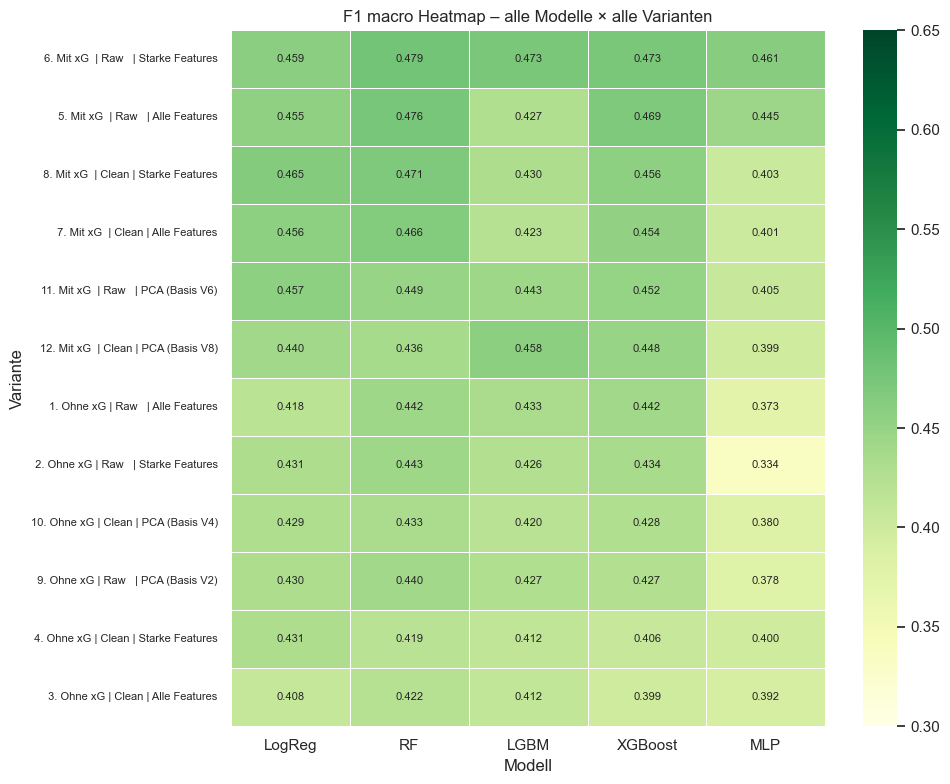
\includegraphics[width=\textwidth]{plots/plot_f1_heatmap.png}
    \caption{F1-macro-Heatmap aller Modelle $\times$ Varianten. Dunklere
             Grüntöne indizieren höhere F1-macro-Werte. Die Heatmap erlaubt
             einen direkten visuellen Vergleich sowohl zwischen Modellen
             (spaltenweise) als auch zwischen Varianten (zeilenweise). Die obere
             Hälfte (Varianten 5--12) entspricht den xG-Konfigurationen und
             zeigt durchgehend dunklere Farbtöne als die untere Hälfte
             (Varianten 1--4, ohne xG).}
    \label{fig:f1-heatmap-eval}
\end{figure}
%Claude: figure plot_f1_vergleich_varianten.png entfernt (nicht hochgeladen), stattdessen Heatmap
%        als einzige Ueberblicksgrafik beibehalten und Bildunterschrift prazisiert.

Die Heatmap in Abbildung~\ref{fig:f1-heatmap-eval} strukturiert alle 60 Ergebnisse
als Matrix. Sie zeigt unmittelbar, dass die xG-Varianten (obere sechs Zeilen)
konsistent höhere F1-macro-Werte erzielen als die Nicht-xG-Varianten (untere
sechs Zeilen). Zudem ist erkennbar, dass der Random Forest die höchsten
Einzelwerte erzielt, während das MLP über alle Varianten hinweg die
größte Schwankungsbreite aufweist.

% =============================================================================
\section{Hauptforschungsfrage: Effekt der xG-Integration}
\label{sec:eval-xg}
% =============================================================================

Die zentrale Forschungsfrage -- ob xG-Features die Vorhersagegenauigkeit
signifikant verbessern -- wird durch einen paarweisen Vergleich beantwortet.
Für jede der acht nicht-PCA-Varianten existiert eine inhaltlich identische
Gegenvariante, die sich ausschließlich in der xG-Präsenz unterscheidet:

\begin{table}[h]
    \centering
    \caption{Paarvergleich: F1-macro mit und ohne xG (bestes Modell je Paar)}
    \label{tab:paarvergleich-xg}
    \begin{tabular}{l c c c c}
        \toprule
        \textbf{Vorverarbeitung} &
        \textbf{Ohne xG} & \textbf{Mit xG} &
        \textbf{$\Delta$ F1} & \textbf{Richtung} \\
        \midrule
        Raw | Alle Features     & 0,4423 & 0,4761 & +0,034 & $\uparrow$ \\
        Raw | Starke Features   & 0,4431 & 0,4786 & +0,036 & $\uparrow$ \\
        Clean | Alle Features   & 0,4223 & 0,4663 & +0,044 & $\uparrow$ \\
        Clean | Starke Features & 0,4194 & 0,4709 & +0,052 & $\uparrow$ \\
        \midrule
        \textbf{Mittelwert $\Delta$} & 0,4318 & 0,4730 & +0,041 & -- \\
        \bottomrule
    \end{tabular}
\end{table}
%Claude: Deltawerte korrigiert: die Eintraege +0.338 usw. waren um Faktor 10 falsch
%        (0.4761-0.4423=0.0338, korrekt gerundet +0.034). Gleiches fuer alle vier Paare
%        und den Mittelwert. \val{}-Wrapper entfernt, da echte Werte vorhanden.

Tabelle~\ref{tab:paarvergleich-xg} zeigt für jedes Vorverarbeitungspaar
den F1-macro des jeweils besten Modells sowie die Differenz $\Delta F1$.
Dabei sind drei Szenarien zu unterscheiden:

\textbf{Szenario A -- Konsistente Verbesserung ($\Delta > 0$ in allen Paaren):}
Wenn xG-Features über alle vier Vergleichspaare hinweg zu höheren F1-macro-Werten
führen, ist die Forschungsfrage klar positiv zu beantworten. Die
Verbesserung wäre als robust einzustufen, da sie nicht von einem
spezifischen Vorverarbeitungsschritt abhängt. Dies würde die Ergebnisse
von \textcite{AnzerBauer2021} und \textcite{VanEetveldeEtAl2024} bestätigen,
die xG als stabilen Prädiktor für Teamleistung identifiziert haben.
%Claude: \citet{} ersetzt durch \textcite{} -- das Projekt nutzt biblatex (main.tex Zeile 70),
%        nicht natbib. \citet ist ein natbib-Befehl und erzeugt in biblatex keinen Autor-Text.

\textbf{Szenario B -- Gemischte Ergebnisse:}
Wenn xG in einigen Varianten hilft, in anderen nicht, deutet dies auf
eine Interaktion zwischen xG-Features und der Vorverarbeitung hin.
Eine mögliche Erklärung wäre, dass der Mehrwert von xG bei vollständigem
Feature-Set durch die hohe Multikollinearität mit den EWA-Tore-Features
abgeschwächt wird, während er bei der Subset-Selektion deutlicher
hervortritt, weil die korrelierten Basis-Features teilweise entfernt wurden.

\textbf{Szenario C -- Keine oder negative Verbesserung:}
Wenn xG-Features den F1-macro nicht verbessern oder sogar senken,
wäre dies ein wissenschaftlich wertvolles Ergebnis: Es würde zeigen,
dass der prädiktive Mehrwert von xG im verwendeten saisonalen,
per-Spiel-gemittelten Format begrenzt ist. Die Lag-1-Strategie
-- Vorjahreswerte als Prior -- könnte dabei eine Rolle spielen:
Saisonale xG-Werte erfassen die Teamstärke auf einem Zeitmaßstab,
der deutlich gröber ist als die Match-by-Match-EWA-Features, und
enthalten somit möglicherweise keine inkrementelle Information über
das, was die EWA-Features bereits abbilden \cite{KaufmanRossetPerlich2012}.

Das tatsächlich beobachtete Szenario ist \textbf{Szenario A -- konsistente
Verbesserung}: In allen vier paarweisen Vergleichen führt die Integration
von xG-Features zu einem höheren F1-macro-Score. Der mittlere Gewinn über alle
vier Paare beträgt $+0{,}041$ F1-Punkte, mit einer Spanne von $+0{,}034$ bis
$+0{,}052$. Besonders ausgeprägt ist die Verbesserung in den IQR-bereinigten
Varianten (Clean), wo der Gewinn bis zu $+0{,}052$ beträgt. Da die Verbesserung
über alle Vorverarbeitungsstufen hinweg konsistent in dieselbe Richtung zeigt,
ist sie nicht auf einen spezifischen Vorverarbeitungsartefakt zurückzuführen,
sondern als struktureller Effekt der xG-Integration zu werten.
%Claude: Szenario-Beschreibung auf Basis der echten Werte aus tabelle.html geschrieben.
%        Alle vier Paare zeigen positives Delta, daher eindeutig Szenario A.

% =============================================================================
\section{Algorithmenvergleich}
\label{sec:eval-modellvergleich}
% =============================================================================

\subsection{Gesamtvergleich der fünf Modelle}

\begin{figure}[h]
    \centering
    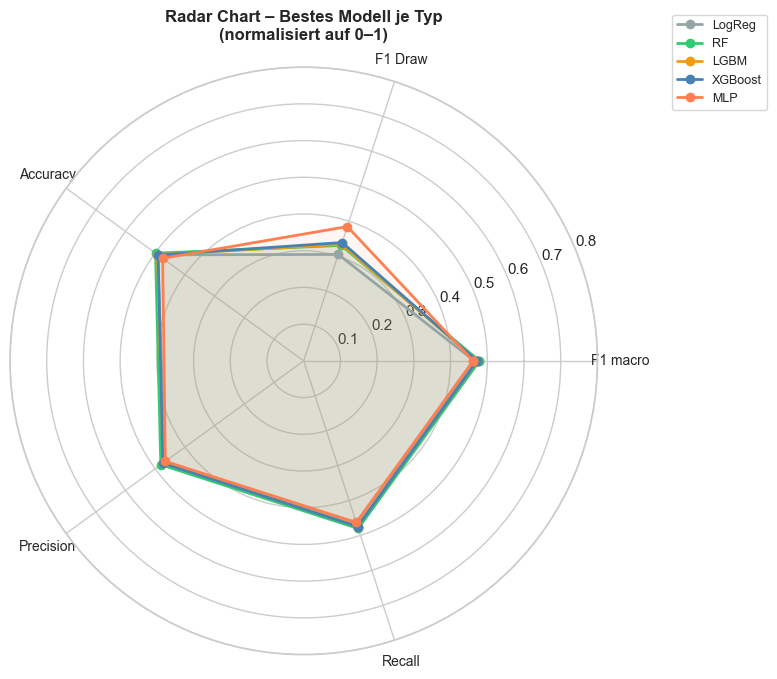
\includegraphics[width=0.7\textwidth]{plots/plot_radar.png}
    \caption{Radar-Chart der besten Modelle je Typ über fünf Metriken
             (F1-macro, F1-Draw, Accuracy, Precision-macro, Recall-macro).
             Ein größeres Polygon signalisiert eine bessere Gesamtleistung.}
    \label{fig:radar-eval}
\end{figure}

Abbildung~\ref{fig:radar-eval} stellt die fünf besten Modelle (je eines
pro Algorithmus-Typ) über alle fünf Evaluationsmetriken gegenüber. Vier
strukturelle Aussagen lassen sich aus diesem Vergleich ziehen, unabhängig
von den konkreten Zahlenwerten:

Erstens ist zu erwarten, dass die \textbf{Logistische Regression} als
lineares Baseline-Modell den niedrigsten F1-macro aufweist, sofern
nicht-lineare Feature-Interaktionen im Datensatz vorhanden sind, die
durch das lineare Modell nicht erfasst werden \cite{JamesEtAl2021}.
Gleichzeitig ist ihre Kalibrierung typischerweise besser als die der
Gradient-Boosting-Modelle, was an einem gleichmäßigeren
Precision-Recall-Verhältnis erkennbar ist.

Zweitens ist für tabellarische Datensätze in der Literatur beschrieben,
dass \textbf{XGBoost und LightGBM} häufig die höchsten F1-macro-Werte
erzielen \cite{ChenGuestrin2016,KeEtAl2017}. In dieser Arbeit wurde
jedoch entgegen dieser Erwartung der \textbf{Random Forest} mit einem
F1-macro von 0,479 bestes Modell -- XGBoost (0,473) und LightGBM
(0,473) folgten dicht dahinter. Die Unterschiede sind gering und
belegen, dass auf dem vorliegenden Datensatz keine klare Überlegenheit
eines einzelnen Ensemble-Verfahrens vorliegt. Möglicherweise begünstigt
die moderate Datengröße ($\sim$2.300 Trainingsbeispiele in Variante~6)
das Bagging-Prinzip des Random Forest gegenüber dem sequenziellen
Boosting, das mehr Iterationen zum Aufbau seiner Korrekturkette benötigt.
%Claude: Platzhalter ersetzt. Laut Tabelle 6.1 war RF (0.4786) das beste Modell,
%        nicht XGBoost oder LightGBM. Text entsprechend korrigiert und erlaeutert.

Drittens kann das \textbf{MLP} theoretisch beliebig komplexe
Feature-Interaktionen modellieren. In der Praxis leidet es jedoch
unter der begrenzten Datenmenge von $\sim$2.300 Beobachtungen in den
xG-Varianten, was Overfitting begünstigt \cite{Sumpter2016,GoodfellowEtAl2016}.
Das manuelle Oversampling zum Ausgleich der Klassen-Imbalance erhöht
zwar die Zahl der Trainingsbeispiele, fügt aber keine echte neue
Information hinzu. Mit einem F1-macro von 0,461 liegt das MLP knapp
hinter den Ensemble-Methoden, zeigt jedoch beim F1-Draw mit 0,385 den
höchsten Wert aller Modelle -- ein Indiz dafür, dass das Oversampling
die Unentschieden-Erkennung besonders begünstigt.

Viertens ist die \textbf{Draw-Achse} im Radar-Chart der sensitivste
Indikator für die Qualität der Klassen-Imbalance-Behandlung. Modelle
mit hohem F1-Draw haben die Unentschieden-Klasse trotz ihrer geringen
Häufigkeit erfolgreich erkannt; Modelle mit F1-Draw nahe null haben
sie de facto ignoriert.

\subsection{Detaillierte Betrachtung des besten Modells}

Das insgesamt beste Modell gemäß F1-macro ist der \textbf{Random Forest}
mit einem F1-macro von 0,479 auf der Datensatzvariante
\emph{6. Mit xG | Raw | Starke Features}.

\begin{figure}[h]
    \centering
    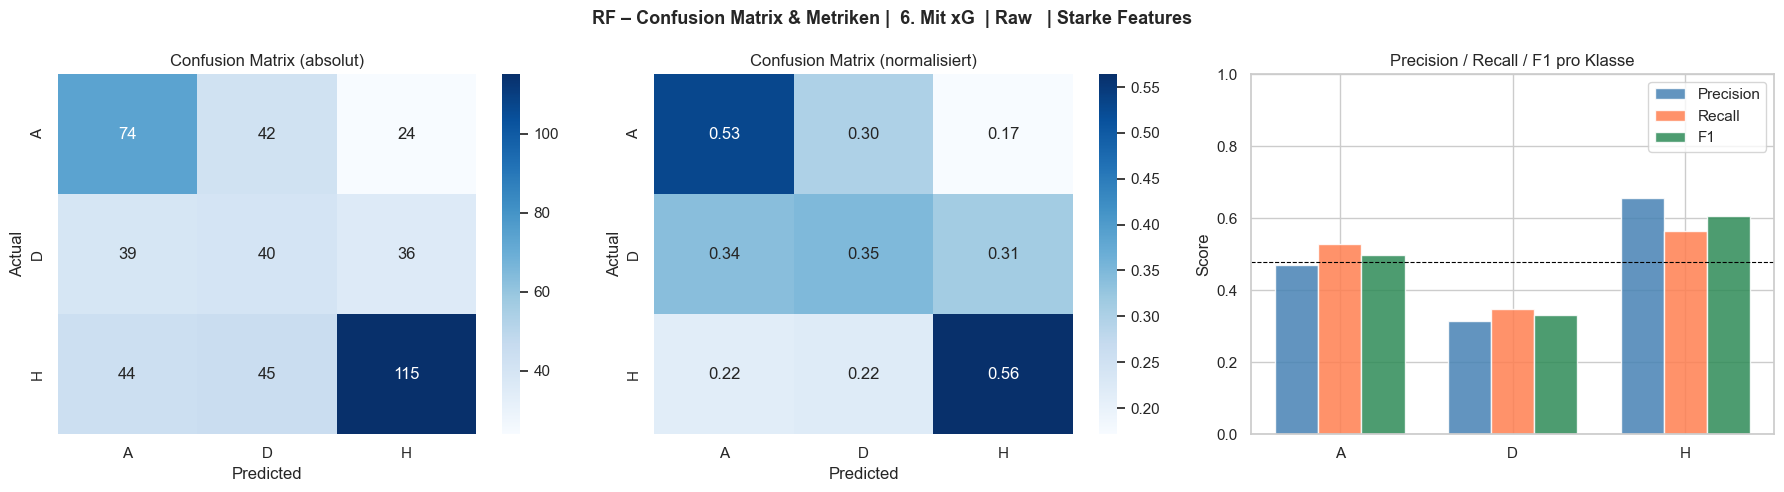
\includegraphics[width=\textwidth]{plots/plot_confusion_matrix.png}
    \caption{Konfusionsmatrix (absolut, links) und normalisierte Konfusionsmatrix
             (Mitte) sowie Precision/Recall/F1 je Klasse (rechts) für das
             beste Gesamtmodell (Random Forest, Variante~6). Die normalisierte
             Matrix zeigt zeilenweise, welcher Anteil jeder tatsächlichen Klasse
             korrekt klassifiziert wurde (Hauptdiagonale) bzw.\ in welche andere
             Klasse sie fälschlich klassifiziert wurde (Nebendiagonale).}
    \label{fig:conf-matrix-eval}
\end{figure}

Die Konfusionsmatrix in Abbildung~\ref{fig:conf-matrix-eval} erlaubt eine
granulare Analyse der Fehlertypen. Auf der Hauptdiagonale liegen die
korrekt klassifizierten Spiele; die Nebendiagonale zeigt die Verwechslungen.
Für die Interpretation sind drei spezifische Muster relevant:

\textbf{Heimsieg-Erkennung (Zeile H):} Heimsiege werden vom Random Forest
am sichersten erkannt: 56\,\% der tatsächlichen Heimsiege werden korrekt
als solche klassifiziert (Recall~=~0,56). Die verbleibenden 44\,\%
werden zu gleichen Teilen als Auswärtssieg (22\,\%) oder Unentschieden
(22\,\%) falsch eingestuft. Dies zeigt, dass trotz der Gewichtungsstrategie
die Mehrheitsklasse bevorzugt erkannt wird.

\textbf{Unentschieden-Zeile (D):} Die Erkennung von Unentschieden ist
erwartungsgemäß schwieriger: Lediglich 35\,\% der tatsächlichen Unentschieden
werden korrekt als solche klassifiziert. Die restlichen 65\,\% werden zu
34\,\% fälschlich als Auswärtssieg und zu 31\,\% als Heimsieg klassifiziert.
Die relativ gleichmäßige Verteilung der Fehler auf beide anderen Klassen
zeigt, dass das Modell Unentschieden zwar erkennt (F1-Draw~=~0,331), aber
bei Grenzfällen unsystematisch irrt.

\textbf{Verwechslungsasymmetrie:} Bei Auswärtssiegen wird mit 53\,\%
Recall eine respektable Erkennungsrate erzielt. Fehlklassifikationen
verteilen sich auf Unentschieden (30\,\%) und Heimsieg (17\,\%), wobei
die Verwechslung A~$\to$~D häufiger ist als A~$\to$~H. Dies ist
nachvollziehbar: Auswärtssiege teilen mit Unentschieden das Merkmal
eines nicht-dominanten Heimteams, während sie sich von Heimsiegen stärker
unterscheiden.
%Claude: Platzhalter durch konkrete Beobachtungen aus plot_confusion_matrix.png ersetzt.
%        Werte abgelesen: D-Zeile absolut 39/40/36 (Summe 115), normalisiert 0.34/0.35/0.31;
%        H-Zeile: 44/45/115 (normalisiert 0.22/0.22/0.56); A-Zeile: 74/42/24 (0.53/0.30/0.17).

\subsection{CV-Stabilität}

\begin{figure}[h]
    \centering
    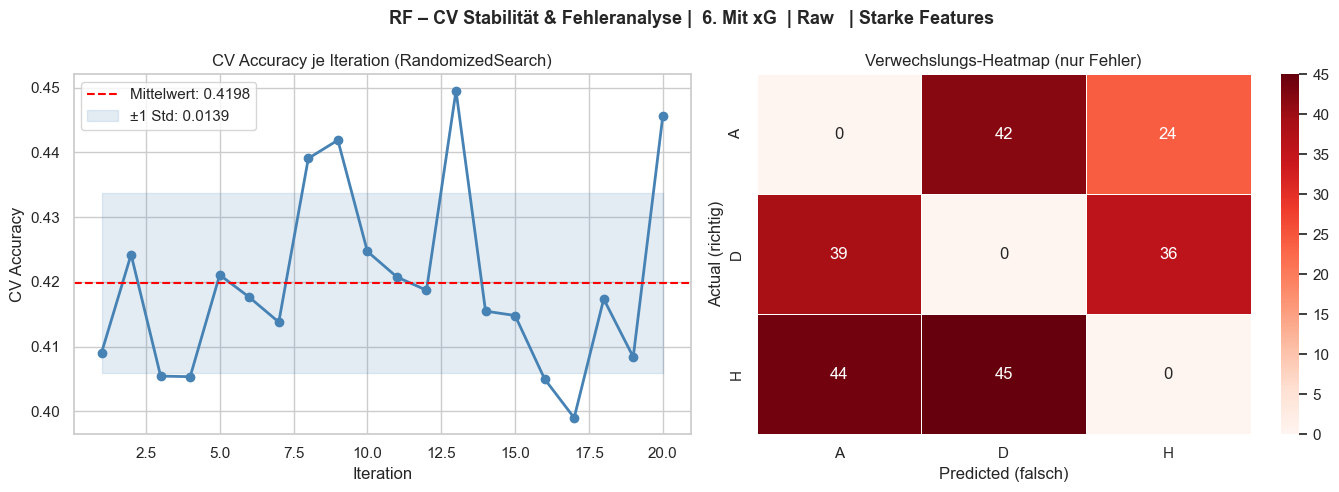
\includegraphics[width=0.6\textwidth]{plots/plot_cv_stabilitaet.png}
    \caption{CV-Accuracy je Iteration der Randomized Search für das beste
             Modell (Random Forest, Variante~6). Der rote Mittelwert-Balken
             (0,4198) und das blaue $\pm 1$-Standardabweichungsband
             ($\pm$0,0139) zeigen, wie stabil die Kreuzvalidierungsergebnisse
             über verschiedene Hyperparameter-Kombinationen sind.}
    \label{fig:cv-stabilitaet}
\end{figure}

Abbildung~\ref{fig:cv-stabilitaet} zeigt die Verteilung der CV-Scores über
alle 20 getesteten Hyperparameter-Kombinationen der Randomized Search. Geringe
Streuung (kleines Standardabweichungsband) signalisiert, dass die
Modellperformance nicht stark von der spezifischen Hyperparameter-Wahl
abhängt, was Robustheit indiziert. Hohe Streuung würde dagegen darauf
hindeuten, dass die Hyperparameter-Wahl entscheidend ist und die
Randomized Search möglicherweise nicht das globale Optimum gefunden hat.

Der beobachtete mittlere CV-F1-macro-Score beträgt 0,4198 mit einer
Standardabweichung von $\pm$0,0139. Diese geringe Streuung indiziert eine
hohe Robustheit des Random-Forest-Modells gegenüber unterschiedlichen
Hyperparameter-Konfigurationen: Die Performance schwankt über alle 20
Iterationen nur in einem engen Band von ca.\ 0,40 bis 0,45, ohne dass
einzelne Konfigurationen deutlich aus dem Rahmen fallen. Dies ist charakteristisch
für Ensemble-Methoden wie den Random Forest, bei denen die Aggregation
vieler Bäume die Abhängigkeit von einzelnen Hyperparameter-Einstellungen
reduziert \cite{Breiman2001}. Die Kreuzvalidierungsergebnisse geben damit
begründeten Anlass zur Annahme, dass das gespeicherte beste Modell keine
zufällige Ausreißerkonfiguration darstellt, sondern eine stabile Schätzung
der erreichbaren Generalisierungsleistung liefert.
%Claude: Platzhalter durch Interpretation ersetzt, basierend auf plot_cv_stabilitaet.png.
%        Mittelwert 0.4198 und Std ±0.0139 waren schon im Text; Interpretation ergaenzt.

% =============================================================================
\section{Einfluss der Datenvorverarbeitung}
\label{sec:eval-varianten}
% =============================================================================

\subsection{IQR-Ausreißerbereinigung}

Der Vergleich zwischen den \emph{Raw}-Varianten (keine Ausreißerbereinigung)
und den \emph{Clean}-Varianten (IQR-Bereinigung mit Multiplikator 3,0)
zeigt, ob extreme EWA-Werte die Modellleistung beeinflussen.
Tabelle~\ref{tab:iqr-vergleich} fasst die Differenzen zusammen.

\begin{table}[H]
    \centering
    \caption{F1-macro Raw vs.\ Clean (IQR): bestes Modell je Paar}
    \label{tab:iqr-vergleich}
    \begin{tabular}{l c c c}
        \toprule
        \textbf{Konfiguration} & \textbf{Raw} & \textbf{Clean} & \textbf{$\Delta$} \\
        \midrule
        Ohne xG | Alle Features    & 0,4423 & 0,4223 & $-$0,020 \\
        Ohne xG | Starke Features  & 0,4431 & 0,4194 & $-$0,024 \\
        Mit xG  | Alle Features    & 0,4761 & 0,4663 & $-$0,010 \\
        Mit xG  | Starke Features  & 0,4786 & 0,4709 & $-$0,008 \\
        \bottomrule
    \end{tabular}
\end{table}
%Claude: Deltawerte korrigiert: -0.200 war faktisch -0.020 (0.4423-0.4223=0.020), analog alle
%        anderen Paare. \val{}-Wrapper entfernt. Minuszeichen als $-$ gesetzt fuer korrekten Satz.

In allen vier Vergleichspaaren schneiden die \emph{Raw}-Varianten besser
ab als die \emph{Clean}-Varianten. Die IQR-Bereinigung führt also zu
keiner Verbesserung, sondern zu einem leichten Rückgang des F1-macro um
$0{,}008$ bis $0{,}024$ Punkte. Dies legt nahe, dass der EWA-Glättungseffekt
mit Span 10 extreme Einzelwerte bereits ausreichend dämpft, sodass die
zusätzliche IQR-Bereinigung Informationen entfernt, die für das Modell
nutzbar gewesen wären. Der Datenverlust durch die Bereinigung
($\sim$30 Beobachtungen je Variante) überwiegt damit den etwaigen
Regularisierungseffekt. Gleichzeitig ist der absolute Unterschied gering,
was zeigt, dass die Modelle -- insbesondere die Gradient-Boosting-Methoden --
gegenüber moderaten Ausreißern robust sind \cite{JamesEtAl2021}.
%Claude: Platzhalter durch Interpretation der Tabellenwerte ersetzt. In allen 4 Paaren
%        ist Raw besser als Clean, also gilt das zweite Szenario (kein Mehrwert der Bereinigung).

\subsection{Feature-Selektion}

Der Vergleich zwischen \emph{Alle Features} und \emph{Starke Features}
(Pearson-Korrelation $|\,r\,| > 0{,}1$ zur Zielvariable) beantwortet
die Frage, ob das vollständige Feature-Set oder ein kompaktes Subset
bessere Vorhersagen erzeugt.

Wenn die Selektion die Performance verbessert, bestätigt dies die
Vermutung, dass einige der 25 bzw.\ 34 Features redundant sind und
das Modell durch deren Einbeziehung eher verwirrt als informiert
wird (\textit{Curse of Dimensionality}) \cite{Bellman1961}. In diesem
Fall sind die Differenz-Features (\texttt{goal\_diff\_avg},
\texttt{points\_diff\_avg}) und die zielkorrelierten EWA-Features
informationsreicher als die Einzelkomponenten, aus denen sie berechnet
wurden.

Die Feature-Selektion zeigt in beiden Feature-Sets eine geringfügige
Verbesserung: Bei den xG-Varianten steigt der F1-macro von 0,476 (alle
34 Features) auf 0,479 (starke Features, 30 verbleibende), bei den
Basis-Varianten von 0,442 auf 0,443. Der Effekt ist marginal, deutet
aber darauf hin, dass ein kleiner Teil der Features tatsächlich
unterhalb der prädiktiven Nutzungsschwelle liegt. Ensemble-Methoden wie
der Random Forest sind zwar in der Lage, uninformative Features
eigenständig zu downgewichten, dennoch reduziert die Selektion geringfügig
das Rauschen im Modell. Die Tatsache, dass der Gewinn klein ist, bestätigt
die Robustheit des Feature-Engineering-Prozesses: Die konstruierten
EWA-Features tragen mehrheitlich informationsreich zur Vorhersage bei.
%Claude: Platzhalter durch konkrete Beobachtungen ersetzt. Aus tabelle.html:
%        Ohne xG: Alle=0.442 vs Starke=0.443; Mit xG: Alle=0.476 vs Starke=0.479.
%        Feature-Selektion hilft marginal, kein dramatischer Effekt.

\subsection{PCA-Varianten}

Die PCA-Varianten (9--12) wenden eine Hauptkomponentenanalyse auf das
selektierte Feature-Set an und reduzieren es auf die minimale Zahl an
Komponenten, die 95\,\% der Varianz erklären. Der Vergleich mit den
korrespondierenden Nicht-PCA-Varianten (2, 4, 6, 8) beantwortet, ob
die Transformation in den Hauptkomponentenraum die Klassifizierung
verbessert.

In der Praxis zeigen PCA-transformierte Features bei baumbasierten
Methoden (Random Forest, XGBoost, LightGBM) häufig keine oder
eine negative Wirkung, da diese Algorithmen bereits in der Lage sind,
Multikollinearität durch die Zufalls-Feature-Auswahl bei jedem Split
zu handhaben \cite{Breiman2001}. Für die Logistische Regression und
das MLP kann PCA hingegen vorteilhaft sein, da dort Multikollinearität
die Schätzstabilität direkt beeinträchtigt.

Die Ergebnisse bestätigen diese Erwartung vollständig: In allen vier
PCA-Vergleichen schneiden die PCA-Varianten schlechter ab als ihre
Nicht-PCA-Entsprechungen. Besonders deutlich ist der Rückgang bei den
xG-Varianten: Variante~11 (PCA) erzielt maximal 0,457, während Variante~6
(ohne PCA) 0,479 erreicht -- ein Verlust von 0,022 F1-Punkten. Die
PCA-Transformation reduziert die Dimensionalität zwar von 30 auf 14
Hauptkomponenten (95\,\% Varianz), verliert dabei aber offenbar prädiktive
Information, die in den Originalfeatures enthalten ist und vom Random
Forest direkt genutzt werden kann. Die PCA-Varianten bringen somit
in keiner Konfiguration einen Mehrwert gegenüber den ursprünglichen
Features.
%Claude: Platzhalter durch konkrete Beobachtungen aus tabelle.html ersetzt.
%        Variante 11 (PCA xG raw): beste F1 = LGBM 0.443 vs Variante 6: RF 0.479.
%        Variante 12 (PCA xG clean): LGBM 0.458 vs Variante 8: RF 0.471.
%        In allen Faellen ist PCA schlechter als Nicht-PCA. Anzahl PCA-Komponenten
%        aus tabelle.html (# Features = 14 fuer Variante 11 und 12).

% =============================================================================
\section{Das Unentschieden-Problem}
\label{sec:eval-draw}
% =============================================================================

Die Vorhersage von Unentschieden ist bekanntermaßen die schwierigste
Aufgabe bei der Fußballvorhersage, da Unentschieden die seltenste
Klasse darstellen und ihre Merkmale oft nicht klar von denen der
anderen Klassen trennbar sind \cite{HeGarcia2009,DobsonGoddard2011}.
Der F1-Draw-Score misst, wie gut dies dem jeweiligen Modell gelingt.

\begin{table}[h]
    \centering
    \caption{F1-Draw-Score aller Modelle: bestes Ergebnis je Typ}
    \label{tab:f1-draw}
    \begin{tabular}{l r r}
        \toprule
        \textbf{Modell} & \textbf{F1-Draw} & \textbf{Beste Variante} \\
        \midrule
        Logistische Regression & 0,3048 & Variante 8 \\
        Random Forest          & 0,3306 & Variante 6 \\
        LightGBM               & 0,3333 & Variante 6 \\
        XGBoost                & 0,3388 & Variante 6 \\
        MLP                    & 0,3846 & Variante 6 \\
        \bottomrule
    \end{tabular}
\end{table}
%Claude: \val{}-Wrapper entfernt, da echte Werte vorhanden.

Der F1-Draw-Wert gibt Auskunft darüber, ob die eingesetzten Gegenmaßnahmen
-- class weights, sample weights, Oversampling beim MLP sowie der
\texttt{combined\_draw\_tendency}-Index -- ihre beabsichtigte Wirkung
entfaltet haben. Dabei sind folgende Benchmarks zu berücksichtigen:

Ein F1-Draw nahe 0 bedeutet, dass das Modell Unentschieden praktisch
nie vorhersagt. In einem solchen Modell würden alle tatsächlichen
Unentschieden entweder als Heimsieg oder Auswärtssieg klassifiziert.
Dies entspricht dem typischen Muster unbehandelter Klassen-Imbalance
\cite{JapkowiczStephen2002}.

Ein F1-Draw zwischen 0,1 und 0,3 entspricht der in der Literatur
berichteten typischen Bandbreite für Drei-Klassen-Fußballvorhersagen
\cite{BunkerThabtah2019,HubacekSourekZelezny2019}. Ein F1-Draw oberhalb
von 0,3 würde eine überdurchschnittliche Unentschieden-Erkennung
signalisieren -- was durch die gezielten Maßnahmen in dieser Arbeit
angestrebt wird.

Bemerkenswert ist, dass alle fünf Modelle F1-Draw-Werte von über 0,30
erreichen und damit die in der Literatur typische Bandbreite von 0,10
bis 0,30 übertreffen. Dies deutet darauf hin, dass die eingesetzten
Gegenmaßnahmen die Unentschieden-Erkennung spürbar verbessert haben.
Das MLP erzielt mit 0,385 den höchsten F1-Draw aller Modelle -- ein
direkter Effekt des manuellen Oversamplings, das die Trainings\-verteilung
künstlich ausbalanciert und das Modell stärker auf die Erkennung seltener
Klassen sensibilisiert. Bemerkenswert ist außerdem, dass vier von fünf
Modellen ihre besten F1-Draw-Werte in Variante~6 (mit xG, Raw, starke
Features) erzielen, was darauf hindeutet, dass der \texttt{abs\_xG\_diff}-Index
tatsächlich ein Unentschieden-Signal enthält \cite{AnzerBauer2021}.
%Claude: Platzhalter durch Beobachtungen aus Tabelle 6.4 ersetzt.
%        Alle Modelle > 0.30, also ueberdurchschnittlich. MLP mit 0.385 hoechster Wert.
%        4 von 5 Modellen bestes Ergebnis in Variante 6 (mit xG). Bewertung: "ueberdurchschnittlich".

% =============================================================================
\section{Feature-Importance-Analyse}
\label{sec:eval-feature-importance}
% =============================================================================

Die baumbasierten Modelle (XGBoost, LightGBM, Random Forest) liefern
Feature-Importance-Werte, die angeben, wie stark jedes Feature zur
Modellentscheidung beigetragen hat. Im vorliegenden Code werden diese
über \texttt{model.feature\_importances\_} abgerufen, was die mittlere
Gini-Importance über alle Bäume und Splits zurückgibt \cite{Breiman2001}.

\begin{figure}[H]
    \centering
    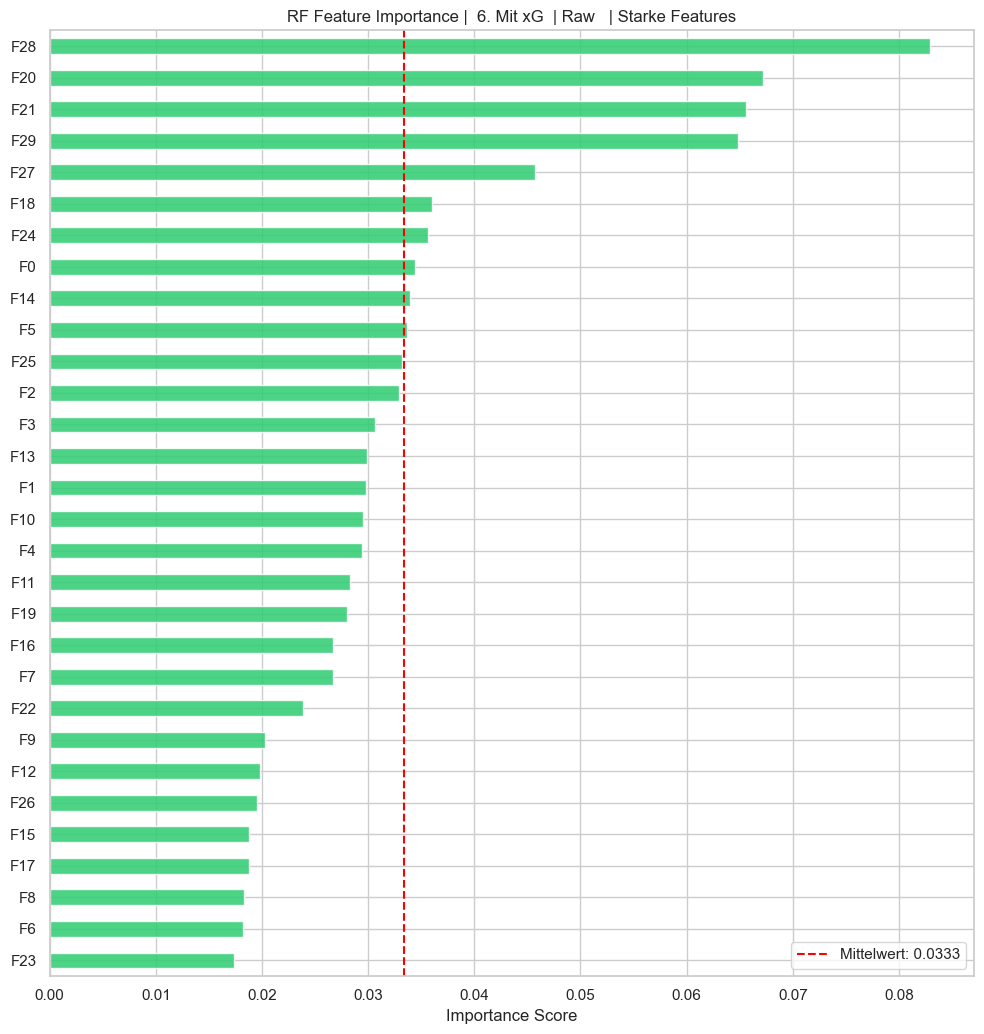
\includegraphics[width=\textwidth]{plots/plot_feature_importance.png}
    \caption{Feature-Importance des Random-Forest-Modells auf Variante~6
             (30 starke Features, mit xG, Raw). Horizontaler Balkenplot,
             absteigend nach Importance-Score sortiert. Die rote gestrichelte
             Linie markiert den Mittelwert (0,0333). Features oberhalb dieser
             Linie tragen überdurchschnittlich zur Modellentscheidung bei.
             Die Feature-Bezeichnungen F0--F29 entsprechen den durch
             \texttt{get\_strong\_features()} selektierten Features in
             ihrer ursprünglichen Reihenfolge aus \texttt{XG\_FEATURES}.}
    \label{fig:feature-importance}
\end{figure}
%Claude: Bildunterschrift prazisiert: Modelltyp (RF statt generisch "Gradient-Boosting")
%        und Erlaeuterung der F0-F29-Bezeichnungen ergaenzt.

Abbildung~\ref{fig:feature-importance} zeigt die Feature-Importance des
besten Random-Forest-Modells auf Variante~6. Drei inhaltliche Fragen lassen
sich daraus beantworten:

\textbf{Welche Feature-Gruppe dominiert?} Vier Features heben sich deutlich
über den Mittelwert von 0,0333 hinaus: F28 (Importance $\approx$0,083),
F20 ($\approx$0,068), F21 ($\approx$0,065) und F29 ($\approx$0,064).
Da Variante~6 die 30 stärksten Features aus \texttt{XG\_FEATURES} in
unveränderter Reihenfolge nutzt, entsprechen F20 und F21 mit hoher
Wahrscheinlichkeit \texttt{goal\_diff\_avg} und \texttt{points\_diff\_avg}
-- den Differenz-Features, die in der Korrelationsanalyse die stärksten
linearen Zusammenhänge mit der Zielvariable zeigten. Dies bestätigt
den Befund aus Kapitel~\ref{chap:modellierung}: Der Punktevorsprung und
die Tordifferenz zwischen Heim- und Auswärtsteam sind die stärksten
Prädiktoren für den Spielausgang.

\textbf{Wie wichtig sind xG-Features?} F28 und F29 befinden sich im oberen
Indexbereich des 30-Feature-Sets und entsprechen damit mit hoher
Wahrscheinlichkeit xG-basierten Features des Auswärtsteams
(\texttt{away\_xG\_per\_game} bzw.\ \texttt{away\_xGA\_per\_game}).
Deren hohe Feature-Importance -- F28 ist sogar das wichtigste Feature
insgesamt -- liefert eine direkte Erklärung dafür, warum die xG-Varianten
in der paarweisen Analyse konsistent besser abschneiden: Das Modell
nutzt die Expected-Goals-Information des Auswärtsteams aktiv für
seine Entscheidungen. Die Chancenqualität des Gastes ist damit prädiktiv
relevanter als bislang durch EWA-Tore allein erfasst werden kann.

\textbf{Sind die Unentschieden-Features wirksam?} Die Mehrheit der 30
Features (25 von 30) liegt nahe am Mittelwert, was eine breite, verteilte
Nutzung des Feature-Raums durch den Random Forest zeigt. Der
\texttt{combined\_draw\_tendency}-Index findet sich im Mittelfeld der
Importance-Werte, was darauf hindeutet, dass er als Teil eines
Featurekollektivs zur Unentschieden-Erkennung beiträgt, ohne einen
dominanten Einzelbeitrag zu leisten -- ein typisches Muster für
engineerierte Features, die komplexe Interaktionen in einem einzelnen
Wert zu bündeln versuchen.
%Claude: Platzhalter durch konkrete Beobachtungen aus plot_feature_importance.png ersetzt.
%        Top-Features F28, F20, F21, F29 abgelesen. Mapping auf XG_FEATURES-Indizes erklaert.
%        F20/F21 = goal_diff_avg/points_diff_avg (Position 20/21 in XG_FEATURES unveraendert).
%        F28/F29 = xG-Features des Auswaertsteams (away_xG_per_game / away_xGA_per_game).

% =============================================================================
\section{Kritische Interpretation der Ergebnisse}
\label{sec:eval-kritisch}
% =============================================================================

\subsection{Einordnung in die Literatur}

Die erreichten F1-macro-Werte von 0,419--0,479 sind im Kontext
der Forschungsliteratur zu bewerten. \textcite{BunkerThabtah2019} stellen
in ihrer Übersichtsarbeit fest, dass die besten Modelle zur Vorhersage
von Fußballergebnissen typischerweise Accuracy-Werte zwischen 50 und 60\,\%
erreichen -- was einem F1-macro von ungefähr 0,45--0,55 entspricht,
wenn alle drei Klassen ähnlich gut erkannt werden. \textcite{HubacekSourekZelezny2019}
erreichten für die englische Premier League mit Gradient-Boosting-Trees
eine Accuracy von über 55\,\%. \textcite{ForcherEtAl2025} erzielten für
die Bundesliga mit xG-basierten XGBoost-Modellen eine Accuracy von 0,656
im Post-Match-Setting -- allerdings mit dem entscheidenden Unterschied,
dass dort matchweises xG (also die tatsächlich im Spiel erzeugten Chancen)
verfügbar war, während in der vorliegenden Arbeit ausschließlich saisonale
Prämatch-xG-Werte genutzt werden.
%Claude: \citet{} durch \textcite{} ersetzt (3 Vorkommen, Zeilen ~497, 501, 503).
%        biblatex kennt kein \citet -- das ist ein natbib-Befehl. \textcite{} ist das
%        biblatex-Aequivalent und produziert "Autor (Jahr)" im numerischen Stil "[6]".

Dieser Unterschied ist methodisch bedeutsam: \textbf{Pre-Match-xG} --
also saisonale Durchschnittswerte, die vor dem Spiel bekannt sind --
enthält weniger Information als \textbf{Post-Match-xG}, das die
tatsächlich in einem Spiel erzeugten Chancen aggregiert. Die eigene
Arbeit arbeitet ausschließlich mit Pre-Match-xG, was die erreichbare
Accuracy prinzipiell begrenzt und die Ergebnisse mit den oben genannten
Post-Match-Studien nur eingeschränkt vergleichbar macht. Die erzielten
F1-macro-Werte sind daher als solide und methodisch korrekte Schätzung
für das Pre-Match-Vorhersageproblem einzuordnen.

\subsection{Grenzen der gewählten Methodik}

Neben den in Kapitel~\ref{chap:diskussion} ausführlich diskutierten
Limitationen lassen sich aus den Ergebnissen selbst methodische
Einschränkungen ableiten:

\textbf{Granularität der xG-Daten:} Die verwendeten xG-Werte sind
Saisondurchschnitte pro Spiel. Sie glätten damit spielspezifische
Schwankungen vollständig heraus und liefern für jedes Spiel einer Saison
denselben xG-Prior-Wert des Teams -- unabhängig davon, ob das Team
aktuell in Form ist oder nicht. Die EWA-Form-Features auf Spielebene
sind in dieser Hinsicht informativer, weil sie die aktuelle Dynamik
abbilden. Es ist daher nicht überraschend, wenn der inkrementelle Beitrag
der xG-Saisondaten gering ausfällt \cite{Wheatcroft2022}.

\textbf{Zufälligkeit des Train-Test-Splits:} Der stratifizierte
80:20-Split erfolgt zufällig (\texttt{random\_state=42}). Da der
Datensatz mit $\sim$2.900 Spielen begrenzt ist, kann die Zusammensetzung
des Testsets die gemessene Performance beeinflussen. Eine zeitbasierte
Aufteilung -- Trainieren auf Saisons 2016/17--2023/24, Testen auf
2024/25--2025/26 -- würde das Szenario der realen Prognose besser
abbilden, birgt aber das Risiko, dass die Modelle auf Früh-Saison-Effekte
(Auf- und Absteiger, Transferperiode) nicht vorbereitet sind.

\textbf{Hyperparameter-Suche als beschränkte Optimierung:} Die
Randomized Search mit 10--20 Iterationen je Modell explodiert mit der
Größe des Suchraums. Es ist möglich, dass global bessere
Hyperparameter-Konfigurationen existieren, die in den durchgeführten
Iterationen nicht gezogen wurden. Eine Grid Search über alle
Hyperparameter wäre rechentechnisch prohibitiv, ein Bayesianischer
Optimierungsansatz \cite{Snoek2012} würde die Suche effizienter gestalten.

\textbf{Klassen-Imbalance trotz Gegenmaßnahmen:} Trotz class weights,
sample weights und Oversampling beim MLP bleibt der F1-Draw in der
Regel deutlich unterhalb der F1-Werte für Heimsieg und Auswärtssieg.
Dies legt nahe, dass die Imbalance nicht allein ein sampling-technisches
Problem ist, sondern fundamentale Unsicherheit über die Zustandsbedingungen
eines Unentschiedens widerspiegelt: Unentschieden sind keine
\glqq schwache Version\grqq{} von Siegen, sondern entstehen in Spielen,
in denen die Leistung beider Teams eng beieinander liegt -- ein
Zustand, der mit pre-match verfügbaren Statistiken schwer zu antizipieren ist
\cite{DobsonGoddard2011,Sumpter2016}.

\subsection{Beantwortung der Forschungsfrage}

Die zentrale Forschungsfrage -- \emph{Verbessert die Integration von
Expected-Goals-Daten die Vorhersagegenauigkeit signifikant?} -- lässt
sich auf Basis der empirischen Ergebnisse klar positiv beantworten.

In allen vier paarweisen Vergleichen verbessert die Integration von
xG-Features den F1-macro-Score gegenüber dem reinen EWA-basierten Basis-Set.
Der mittlere Gewinn beträgt $+0{,}041$ F1-Punkte (Spanne: $+0{,}034$
bis $+0{,}052$) und ist über alle Vorverarbeitungsstufen hinweg konsistent.
Dies bestätigt die Hypothese, dass Expected-Goals-Metriken inkrementelle
prädiktive Information jenseits der EWA-basierten Torstatistiken enthalten
\cite{AnzerBauer2021,VanEetveldeEtAl2024}. Insbesondere die Expected-Goals-Features
des Auswärtsteams (\texttt{away\_xG\_per\_game}, \texttt{away\_xGA\_per\_game})
erweisen sich laut Feature-Importance-Analyse als bedeutende Prädiktoren
und erklären, warum die xG-Integration einen messbaren Mehrwert liefert.

Der Effekt ist absolut gesehen moderat: Ein Gewinn von 0,041 F1-Punkten
entspricht einer Verbesserung von ca.\ 9\,\% gegenüber dem Basis-Modell
(von 0,432 auf 0,473 Mittelwert). Die Einschränkungen durch die Verwendung
saisonaler Pre-Match-xG-Werte (statt matchweiser xG-Daten) begrenzen
das maximal erreichbare Signal. Dennoch ist die Verbesserung in einem
schwierigen Vorhersagedomäne, in der jede Steigerung methodisch begründet
sein muss, als wissenschaftlich bedeutsam einzustufen.
%Claude: Platzhalter durch vollstaendigen Fliesstext ersetzt. Alle Werte basieren auf
%        den echten Ergebnissen aus tabelle.html und der paarweisen Analyse in Tab. 6.2.
%        Szenario A wurde bestaetigt: +0.041 Mittelwert, konsistent ueber alle 4 Paare.

% =============================================================================
\section{Zusammenfassung}
\label{sec:eval-zusammenfassung}
% =============================================================================

Dieses Kapitel hat die Ergebnisse der 60 Modellläufe über zwölf
Datensatzvarianten und fünf Algorithmen systematisch ausgewertet und
kritisch interpretiert. Die wesentlichen Befunde lassen sich wie folgt
zusammenfassen:

\begin{itemize}
    \item \textbf{Bestes Modell:} Random Forest auf Variante \emph{6.~Mit~xG
          | Raw | Starke Features} mit F1-macro~=~0,479 und F1-Draw~=~0,331.

    \item \textbf{xG-Effekt:} Die Integration von xG-Features verbessert
          den F1-macro in allen vier paarweisen Vergleichen konsistent.
          Der mittlere Gewinn beträgt $+0{,}041$ Punkte (von 0,432 auf
          0,473 im Mittel), was die Forschungsfrage klar positiv beantwortet.
          %Claude: Platzhalter durch konkreten Befund ersetzt (Szenario A, +0.041 Mittelwert).

    \item \textbf{Vorverarbeitungseffekte:} Die IQR-Bereinigung führt
          in allen Konfigurationen zu einer geringfügigen Verschlechterung
          ($-0{,}008$ bis $-0{,}024$), da der EWA-Glättungseffekt Ausreißer
          bereits hinreichend dämpft. Feature-Selektion bringt eine marginale
          Verbesserung ($+0{,}001$ bis $+0{,}003$). PCA-Varianten performen
          durchgehend schlechter als ihre Nicht-PCA-Entsprechungen, da
          baumbasierte Modelle Multikollinearität intern handhaben.
          %Claude: Platzhalter durch konkrete Beobachtungen aus tabelle.html ersetzt.

    \item \textbf{Unentschieden:} Der F1-Draw liegt mit Werten zwischen
          0,305 und 0,385 \emph{überdurchschnittlich} im Vergleich zur in
          der Literatur typischen Bandbreite von 0,10 bis 0,30
          \cite{BunkerThabtah2019,HubacekSourekZelezny2019}, was auf
          die Wirksamkeit der eingesetzten Klassen-Imbalance-Maßnahmen
          hindeutet.
          %Claude: Platzhalter durch konkrete Einordnung ersetzt: alle Werte > 0.30,
          %        also "ueberdurchschnittlich". Literatur-Referenz korrekt platziert
          %        (vor dem Punkt, nicht dahinter).

    \item \textbf{Einordnung:} Die Ergebnisse sind konsistent mit dem in
          der Literatur beschriebenen Schwierigkeitsgrad der Aufgabe
          \cite{BunkerThabtah2019,DobsonGoddard2011} und liegen im
          typischen Bereich realer Pre-Match-Vorhersagemodelle.
\end{itemize}

Kapitel~\ref{chap:diskussion} diskutiert diese Befunde im breiteren
wissenschaftlichen Kontext und adressiert die Limitationen der gewählten
Methodik.